\documentclass[10pt, hyperref={unicode}]{beamer}

\usepackage[czech]{babel}
\usepackage[utf8]{inputenc}
\usepackage{times} % font
\usepackage{listings} % algoritmy
\usepackage{xcolor} % definice vlastních barev
\usepackage{graphics} % vkládání obrázků
\usepackage[T1]{fontenc}
\usepackage[utf8]{inputenc}
\usepackage{url}
\usetheme{Goettingen}
\usecolortheme{seahorse}

% číslování aktuální snímek/celkem snímků
\setbeamertemplate{footline}[frame number]

\AtBeginSection[]
{
    \begin{frame}
        \frametitle{Následující sekce}
        \tableofcontents[currentsection]
    \end{frame}
}


\title{Hashovací tabulky}
\subtitle{ITY\,--\,5. Projekt}
\author{Hana Liškařová}
\institute
{
 Vysoké učení technické v~Brně\\
 FIT
}

\date{\today}

\begin{document}

\frame{\titlepage}

\begin{frame}{Obsah}
\frametitle{Obsah prezentace}
\tableofcontents
\end{frame}

\section{Definice}

\begin{frame}{Co je to hashovací tabulka?}
    \begin{itemize}
        \item \uv{Vyhledávací datová struktura, která asociuje hašovací klíče s odpovídajícími hodnotami. Hodnota klíče je spočtena z obsahu položky pomocí nějaké hašovací funkce}
        \item Datová struktura pro ukládání dvojic \alert{(klíč, hodnota)}
        \item Dobrý kompromis mezi rychlostí vyhledávání a paměťovou náročností
    \end{itemize}
    
\end{frame}
\section{Princip funkce}

\begin{frame}{Funkce}
    \begin{enumerate}
        \item Hashování klíče
        \begin{itemize}
            \item klíč je převeden na index v poli pomocí hashovací funkce
        \end{itemize}

        \item Uložení do pole
        \begin{itemize}
            \item prvek je umístěn do pole na získaném indexu
        \end{itemize}

        \item Kolize
        \begin{itemize}
            \item pokud dva různé klíče mají stejný hash, dochází ke kolizi
            \item Řešení: například pomocí řetězcování, otevřeného adresování nebo perfektního hashování
        \end{itemize}
    \end{enumerate}
    
\end{frame}

\begin{frame}{Funkce}

    \begin{columns}[T]
    \begin{column}{.6\textwidth}

        \begin{enumerate}
        
        \item Vyhledání
        \begin{itemize}
            \item klíč je opět převeden na index
            \item prvek na daném indexu je porovnán s hledaným klíčem
        \end{itemize}

        \item Odstranění
        \begin{itemize}
            \item prvek s odpovídajícím klíčem je odstraněn z pole
        \end{itemize}
    \end{enumerate}

    \end{column}
    \begin{column}{.4\textwidth}

    \begin{figure}
        \centering
        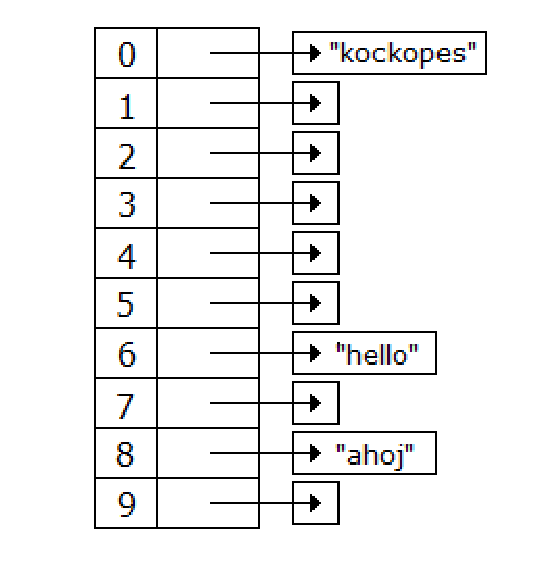
\includegraphics[width=1\linewidth]{hash.pdf}
        \caption{Hashovací tabulka}
        \label{Obrazek 1}
    \end{figure}
    \end{column}
  \end{columns}
    
    
\end{frame}
        

\section{Operace}
\begin{frame}{Operace nad Hashovacími tabulkami}

    \begin{enumerate}
        \item Vkládání (Insertion)
        \begin{itemize}
            \item výpočet indexu pomocí klíce a hash funkce
            \item pokud je cílový index volný, je prvek uložen
        \end{itemize}

        \item Vyhledávání (Search)
        \begin{itemize}
            \item výpočet indexu pomocí klíce a hash funkce
            \item prvek na získaném indexu je porovnán s hledaným prvkem
        \end{itemize}

        \item Odstranění (Deletion)
        \begin{itemize}
            \item výpočet indexu pomocí klíce a hash funkce
            \item prvek na získaném indexu je odstraněn, pokud existuje.
        \end{itemize}
    \end{enumerate}
    
\end{frame}
\subsection{Ukázky pseudokódu}
\begin{frame}[fragile]{Ukázky pseudokódu}

    \begin{lstlisting}[title=Function for creating and initializing a hash table]
    function create_hash_table(size):
        hash_table = new Array(size)
        for i from 0 to size - 1:
            hash_table[i] = new LinkedList()
    return hash_table
\end{lstlisting}

\begin{lstlisting}[title=Function to retrieve a value from the hash table given a key]
    function get(hash_table, key):
        index = hash_function(key, size_of(hash_table)) 
        list_at_index = hash_table[index]  
        for each pair in list_at_index:
            if pair.key equals key:
                return pair.value
        return null  
\end{lstlisting}

    
\end{frame}

\begin{frame}[s]
    \vfill
    \centering \Large Děkuji za pozornost
    \vfill
\end{frame}

\begin{frame}{Zdroje}
    \bibliographystyle{czechiso}
    \bibliography{proj5}
\end{frame}


\end{document}
